\chapter{General discussion}
\label{chap:general-discussion}

\section{A prototype for landscape-scale phenotyping}

\begin{figure}[H]
    \centering
    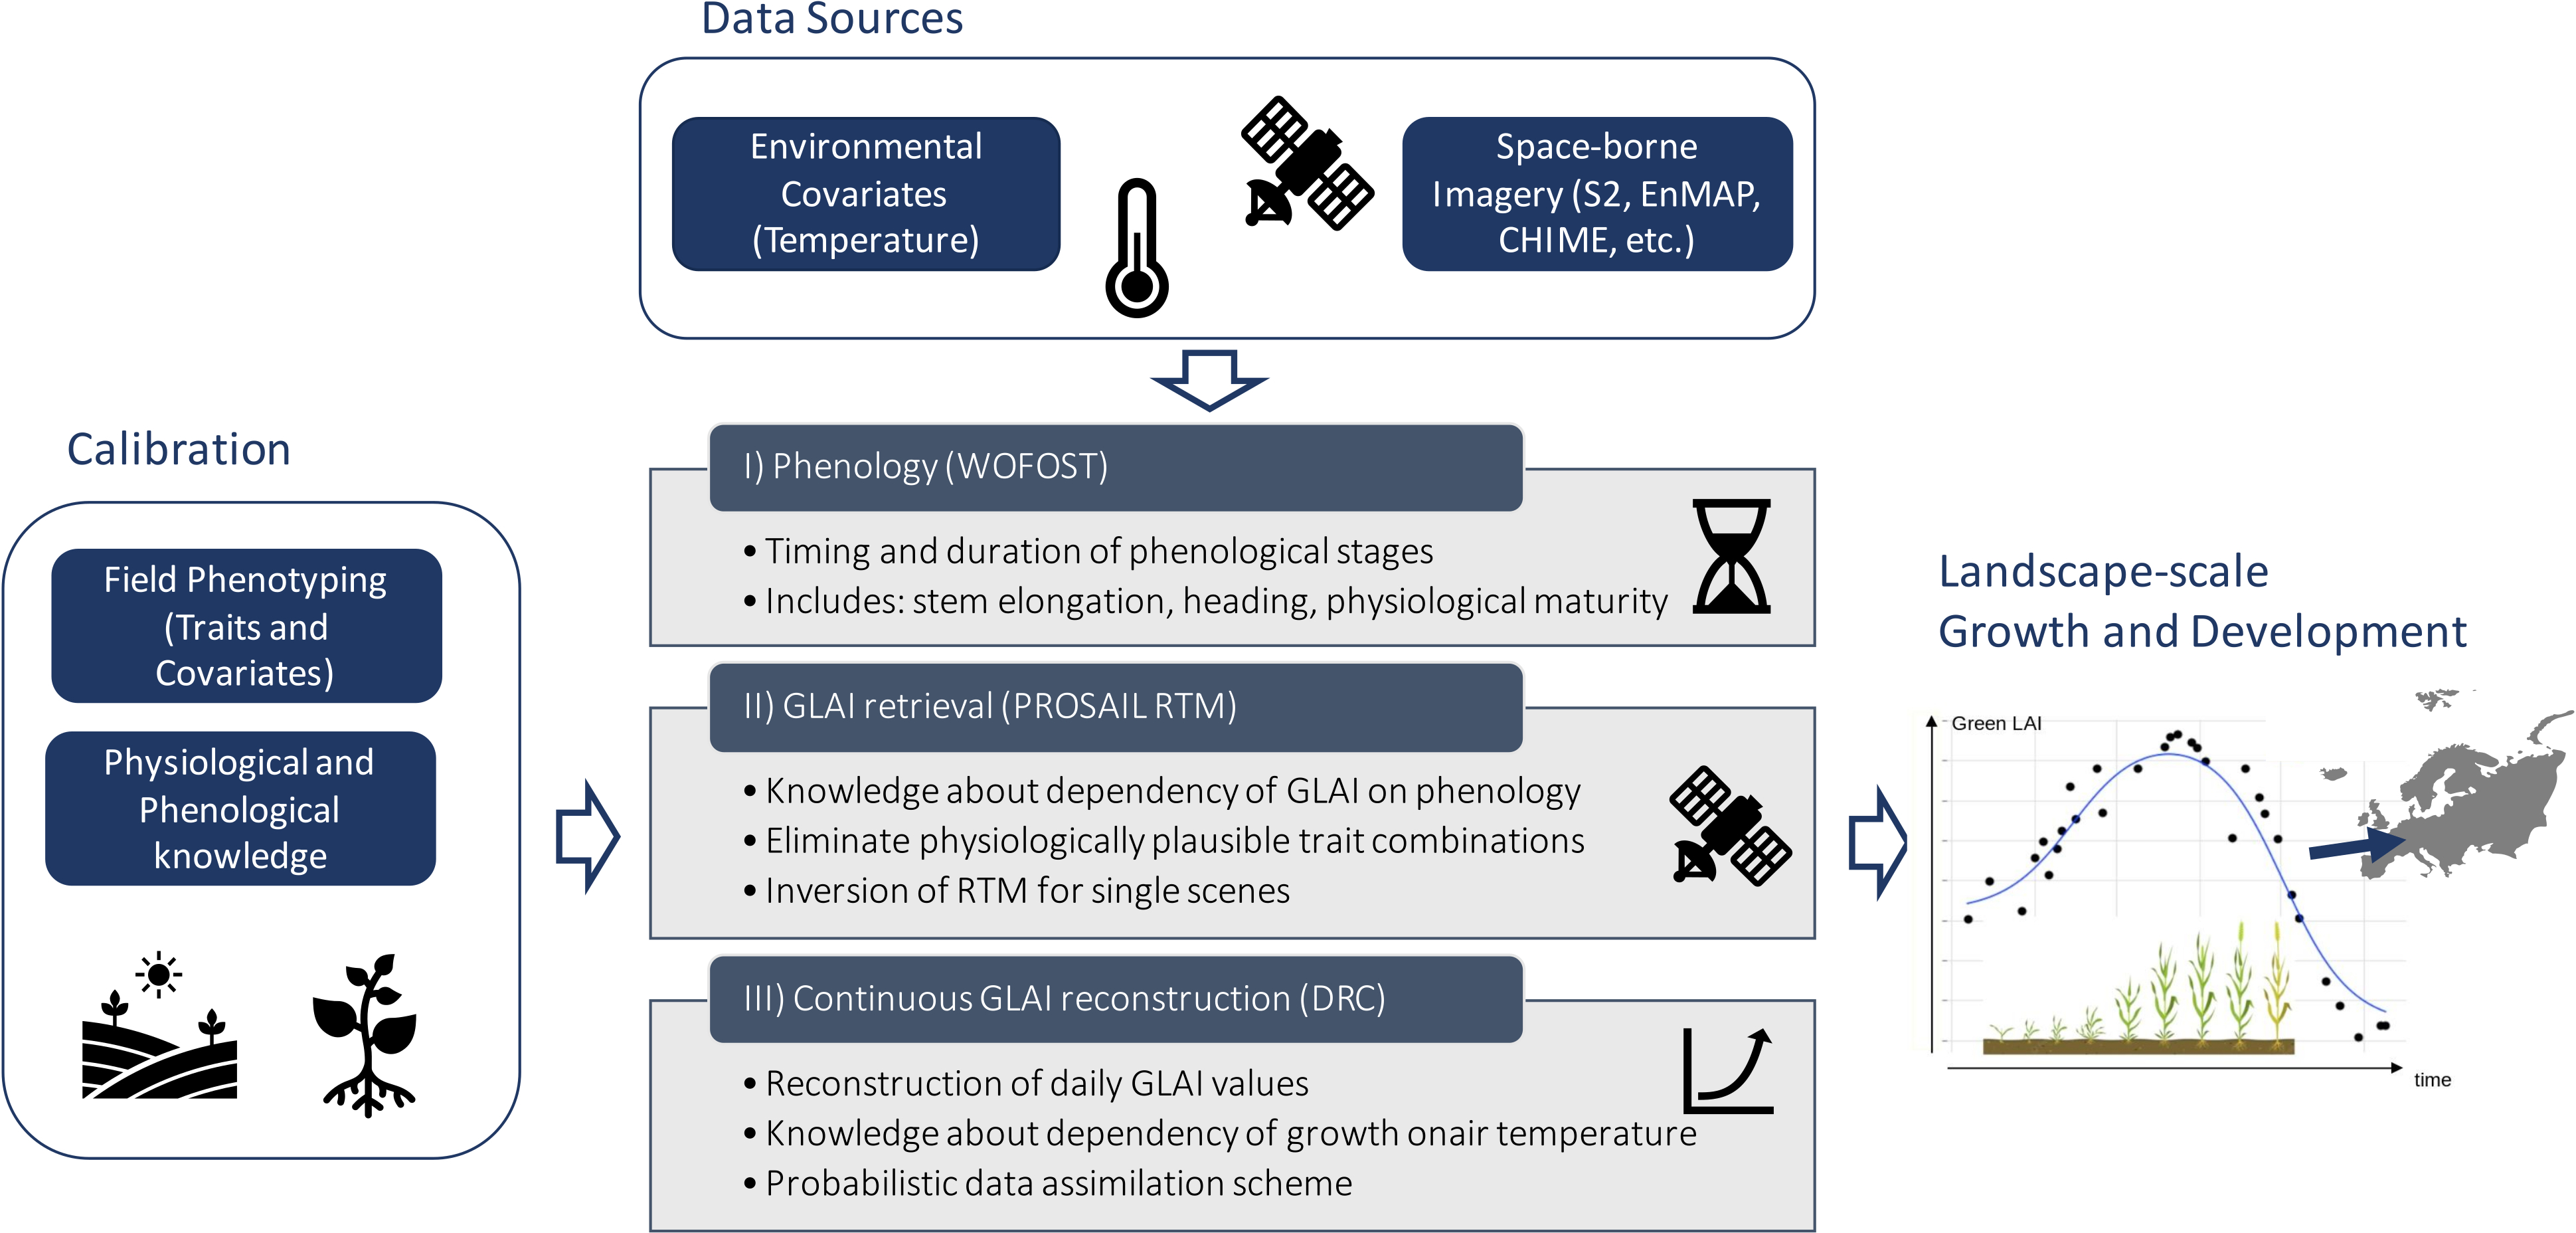
\includegraphics[width=\textwidth]{07-Discussion/img/prototype.jpg}
    \caption{The proposed prototype for landscape scale phenotyping of winter wheat growth and development as a key outcome of this thesis.}
    \label{fig:oa-disc-prototype}
\end{figure}

\section{Open questions}
% open question future academic work could address
% what is more important: spatial or temporal resolution? -> S2-L8 example -> what is the "right" resolution
% which parts of the growth period are the most crucial, e.g., for data assimilation -> I argue that we should do it like the breeders and pay most attention to the critical transitions

\section{Current limitations and ways forward}
% mainly limitations for an operational usage of the proposed system but also scientifically relevant at larger spatial scales
\subsection{Data}
% lack of in-season crop and cultivar information
% poor management information (sowing dates)
% lack of in-situ cal/ val data
\subsection{Methods}
% more explicit linkage to agronomically relevant traits such as yield or nitrogen-/ water-use efficiency for policy making & enforcement
% more complex DRC like Wang Engels and phenology model also for stem elongation -> flavian
% extend to other crops -> flavian
